\documentclass{standalone}
\usepackage{graphicx}	
\usepackage{amssymb, amsmath, amsthm}
\usepackage{color}

\usepackage{tikz}
\usetikzlibrary{arrows.meta, math}

\definecolor{light}{RGB}{220, 188, 188}
\definecolor{mid}{RGB}{185, 124, 124}
\definecolor{dark}{RGB}{143, 39, 39}
\definecolor{highlight}{RGB}{180, 31, 180}
\definecolor{lightteal}{RGB}{107, 142, 142}
\definecolor{midteal}{RGB}{72, 117, 117}
\definecolor{darkteal}{RGB}{29, 79, 79}
\definecolor{gray10}{gray}{0.1}
\definecolor{gray20}{gray}{0.2}
\definecolor{gray30}{gray}{0.3}
\definecolor{gray40}{gray}{0.4}
\definecolor{gray60}{gray}{0.6}
\definecolor{gray70}{gray}{0.7}
\definecolor{gray80}{gray}{0.8}
\definecolor{gray90}{gray}{0.9}
\definecolor{gray95}{gray}{0.95}

\newcommand{\arrow}[5]{
  \pgfmathsetmacro{\rx}{#3 - #1}
  \pgfmathsetmacro{\ry}{#4 - #2}
  \pgfmathsetmacro{\n}{sqrt( \rx * \rx + \ry * \ry )}
  
  \pgfmathsetmacro{\vx}{\rx / \n}
  \pgfmathsetmacro{\vy}{\ry / \n}

  \pgfmathsetmacro{\wx}{\vy}
  \pgfmathsetmacro{\wy}{-\vx}  

  \pgfmathsetmacro{\g}{0.01}
  \pgfmathsetmacro{\gx}{-\g * \wx}
  \pgfmathsetmacro{\gy}{-\g * \wy}  
  
  \draw[#5, line width=0.75] 
       (#1 + \gx + 0.75 * \g * \vx, #2 + \gy + 0.75 * \g * \vy) 
    -- (#3 + \gx - 0.75 * \g * \vx, #4 + \gy - 0.75 * \g * \vy); 
    
  \pgfmathsetmacro{\p}{30}
  \pgfmathsetmacro{\d}{0.125}
  \pgfmathsetmacro{\e}{0.04}
  \pgfmathsetmacro{\lx}{#3 - (\d + \e * tan(\p)) * \vx - \e * \wx}
  \pgfmathsetmacro{\ly}{#4 - (\d + \e * tan(\p)) * \vy - \e * \wy}  
  \pgfmathsetmacro{\mx}{#3 - \d * \vx}
  \pgfmathsetmacro{\my}{#4 - \d * \vy}  
  
  \fill[#5]    (#3 + \gx - 0.75 * \g * \vx, #4 + \gy - 0.75 * \g * \vy) 
            -- (\lx + \gx, \ly + \gy)
            -- (\mx + \gx, \my + \gy) 
            -- cycle;
}

\begin{document}

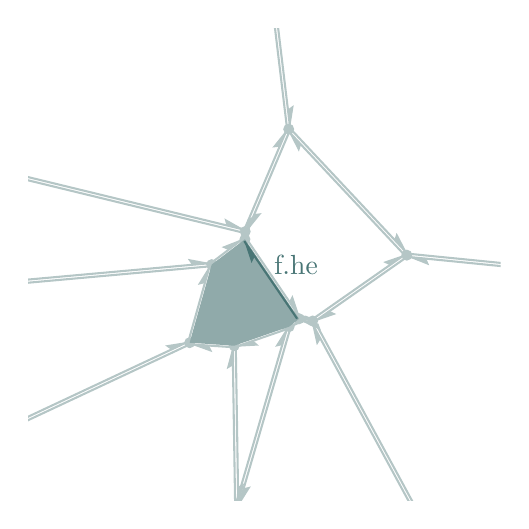
\begin{tikzpicture}[scale=2]
  \draw[white] (-1.5, -1.5) rectangle (1.5, 1.5);
  \clip (-1.5, -1.5) rectangle (1.5, 1.5);
  
  \colorlet{custom}{lightteal!50!white};
  
  % 7
  \foreach \x/\y 
    [remember=\x as \xi (initially -0.475)] [remember=\y as \yi (initially -0.497)] 
    in {-0.192/-0.516, 0.157/-0.395, 0.220/-0.345, -0.124/0.160, 
        -0.335/-0.001, -0.475/-0.497} {
      \arrow{\xi}{\yi}{\x}{\y}{custom}
  };
  
  % 3
  \foreach \x/\y 
    [remember=\x as \xi (initially -0.251)] [remember=\y as \yi (initially -2.000)] 
    in {-0.176/-1.538, -0.192/-0.516, -0.475/-0.497, -2.000/-1.212} {
      \arrow{\xi}{\yi}{\x}{\y}{custom}
  };

  % 9
  \foreach \x/\y 
    [remember=\x as \xi (initially 1.197)] [remember=\y as \yi (initially -2.000)] 
    in {0.306/-0.359, 0.220/-0.345, 0.157/-0.395, -0.176/-1.538, -0.251/-2.000} {
      \arrow{\xi}{\yi}{\x}{\y}{custom}
  };
  
  % 4
  \foreach \x/\y 
    [remember=\x as \xi (initially 2.000)] [remember=\y as \yi (initially -0.050)] 
    in {0.904/0.059, 0.306/-0.359, 1.197/-2.000} {
      \arrow{\xi}{\yi}{\x}{\y}{custom}
  };
  
  % 5
  \foreach \x/\y 
    [remember=\x as \xi (initially 0.017)] [remember=\y as \yi (initially 2.000)] 
    in {0.154/0.859, 0.904/0.059, 2.000/-0.050} {
      \arrow{\xi}{\yi}{\x}{\y}{custom}
  };
  
  % 1
  \foreach \x/\y 
    [remember=\x as \xi (initially -2.000)] [remember=\y as \yi (initially 0.666)] 
    in {-0.122/0.209, 0.154/0.859, 0.017/2.000} {
      \arrow{\xi}{\yi}{\x}{\y}{custom}
  };
  
  % 6
  \foreach \x/\y 
    [remember=\x as \xi (initially -2.000)] [remember=\y as \yi (initially -0.151)] 
    in {-0.335/-0.001, -0.124/0.160, -0.122/0.209, -2.000/0.666} {
      \arrow{\xi}{\yi}{\x}{\y}{custom}
  };
  
  % 2
  \foreach \x/\y 
    [remember=\x as \xi (initially -2.000)] [remember=\y as \yi (initially  -1.212)] 
    in {-0.475/-0.497, -0.335/-0.001, -2.000/-0.151} {
      \arrow{\xi}{\yi}{\x}{\y}{custom}
  };
  
  % 8
  \foreach \x/\y 
    [remember=\x as \xi (initially -0.122)] [remember=\y as \yi (initially 0.209)] 
    in {-0.124/0.160, 0.220/-0.345, 0.306/-0.359, 0.904/0.059, 0.154/0.859, -0.122/0.209} {
      \arrow{\xi}{\yi}{\x}{\y}{custom}
  };
  
  % 10
  \foreach \x/\y 
    [remember=\x as \xi (initially -0.176)] [remember=\y as \yi (initially -1.538)] 
    in {0.157/-0.395, -0.192/-0.516, -0.176/-1.538} {
      \arrow{\xi}{\yi}{\x}{\y}{custom}
  };
  
  \foreach \x/\y 
    in {-0.475/-0.497, -0.335/-0.001, -0.192/-0.516, 
        -0.124/0.160, -0.122/0.209, 0.157/-0.395, 
        -0.176/-1.538, 0.220/-0.345, 0.306/-0.359, 
        0.154/0.859, 0.904/0.059} {
      \fill[custom] (\x, \y) circle (0.035);
  };
  
  
  \colorlet{custom}{lightteal!75!white};
  
  \fill[custom] (-0.475, -0.497)
  \foreach \x/\y in {-0.192/-0.516, 0.157/-0.395, 0.220/-0.345, -0.124/0.160, 
        -0.335/-0.001, -0.475/-0.497} {
      -- (\x, \y)
  };
  
  \arrow{0.220}{-0.345}{-0.124}{0.160}{midteal}
  \node[midteal] at (0.2, 0) { f.he };

\end{tikzpicture}

\end{document}  